\chapter{Protocol of work so far}

\section{Rotated lines experiment}

\subsection{Introduction}

The goal of this task was to recreate experiment 2 from \citet{nessler}.


\subsection{Methods}
Input data:
The images used in this task were 29 x 29 pixel black and white images of lines going through the center of the image. During the training of the network these images are generated and randomly oriented for each training step. To simulate noise each pixel has a ten percent chance to have its color flipped. To ensure that all lines in the images have the same length regardless of their orientation a circular mask with a radius of 15 pixel was applied to the images. This recolors all pixel outside of the mask to white. Two examples of such images can be seen in figure \ref{fig:angleImages}.

\begin{figure}
  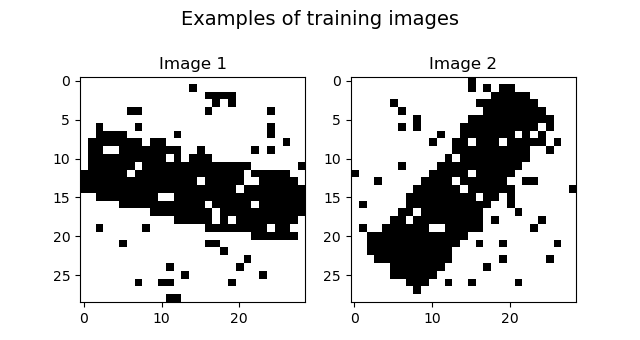
\includegraphics[width=\linewidth]{figures/angleNetwork/trainingImages.png}
  \caption{Two examples of the generated training data in this experiment.}
  \label{fig:angleImages}
\end{figure}

Excitatory input:
The intrinsic weights of the x neurons were omitted in this experiment. This was chosen because there was no benefit in including them.
\begin{equation}
\label{eqn:uk}
U_k(t) = \sum_{i=,}^n w_{ki} \cdot x_i(t)
\end{equation}

Firing rate:
\begin{equation}
\label{eqn:rk}
r_k(t) = e^{u_k(t) - I(t)}
\end{equation}

Chance to spike within time step $\delta t$:
\begin{equation}
\label{eqn:rkdt}
r_k(t) \cdot \delta t
\end{equation}

Weight updates:
\begin{equation}
\label{deltawki}
\Delta w_{ki} = \begin{dcases*} ce^{-w_{ki}} - 1 & if $x_{i}(t^f) = 1$, i.e.$x_{i}$ fired in $ [t^f - \sigma, t^f] $ \\
-1 & \text{if $ y_i(t^f) = 0 $, i.e. $ y_i $ did not fire in $ [t^f - \sigma, t^f] $ } \end{dcases*}
\end{equation}